I primi esperimenti con raggi cosmici diedero evidenza del positrone, così mostrarono l'esistenza di una nuova particella: il 
 \textbf{muone}, $\mu$, $m_\mu=105\,MeV$. Sta in uno stato intermedio tra la massa di un elettrone e protone. Con il suo \textbf{neutrino}. Questa particella è importante per la comprensione delle interazioni deboli: \textbf{famiglie} ed \textbf{universalità}. L'origine dei muoni osservati sulla superficie terrestre si può far risalire al decadimento di un'altra particella: il \textbf{pione}, $\pi$. Osservazione con emulsioni nucleare in voli sul pallone. Particella mediatrice di interazioni forti tra protoni e neutroni che compongono il nucleo: il primo \textbf{mesone}.
 \subsection{Raggi cosmici}
 Sono principalmente nuclei accelerati da sorgenti astrofisiche. La parte bassa dello spettro dei raggi cosmici è dominata da nuclei di origine solare (vento solare). La maggioranza di nuclei che arrivano sulla terra sono protoni. In pratica i raggi cosmici sono costituiti da nuclei che interagiscono già negli stati più alti dell'atmosfera. La sezione d'urto è abbastanza grande da garantire questo. Le interazioni con un nucleo nell'atmosfera vengono prodotte numeroso particelle secondarie (protoni neutroni ma anche pioni) che interagiscono con altri nuclei dell'atmosfera producendo sciami di particelle che interagiscono forte (quindi contenete protoni, neutroni o mesone $\pi$), possono contenere sciami elettromagnetici prodotti da elettroni o fotoni ad alta energia (processo di produzione coppie e Bremsstrahlung). Una parte di questa radiazione prodotta dal decadimento di pioni carichi si trasformano in muoni che possono arrivare sulla superficie terrestre. 
 \subsection{Decadimento del muone}
 Il muone decade con una vita media di $\tau_\mu=2.2\,\mu s$. L'elettrone è l'unica particella carica più leggera del muone quindi forzatamente il muone decate in elettrone. Le altre particelle sono invisibili come il $\nu$. Lo spettro dell'elettrone prodotto dal decadimento del muone. L'energia dell'elettrone ha un endpoin intorno a $50\,MeV$ ed ha uno spettro continuo quindi è per forza un decadimento a tre corpi:
 \begin{equation*}
     \mu^-\to e^-+\Bar{\nu}+\nu
 \end{equation*}
 %IMMAGINE ds
\begin{figure}[htp!]
  \centering
  
\includegraphics[scale=0.45]{Lezione13/ds.png} 
\end{figure}
Un'altra evidenza è che la somma di tre particelle con spin semi-intero da lo spin ancora semi-intero di conseguenza \textbf{il muone è un fermione} e cioè ha spin semi-intero questo perchè il muone decade in 3 corpi con spin semi-intero e quindi anche lei avrà spin semi-intero. La forma esatta dello spettro di energia dell'elettrone dipende dai dettagli dell'elemento di matrice: infatti anche solo guardando lo spettro è molto diverso da quello del decadimento $\beta$. Questo è collegato al fatto che un effetto importante è l'elicità. Infatti nelle interazioni deboli l'elicità è ben definita o per lo meno è diversa da zero. In particolare il caso in cui abbiamo l'elettrone che ha il massimo dell'energia significa che l'elettrone sta rinculando rispetto alle altre particelle. Caso in cui ho di fatto un massimo sbilanciamento dell'energia. Se neutrino e antineutrino vanno nella direzione opposta, i loro spin sono in direzione opposta quindi per bilanciare il momento angolare l'elettrone deve avere direzione dello spin opposta alla direzione del moto e quindi elicità negativa. Noi vediamo che questa configurazione ha alta probabilità di avvenire (picco dello spettro). 

Nel caso in cui l'elettrone porta con se poco momento, significa che il grosso del momento è portato dai neutrini. Quindi neutrino e antineutrino vanno a direzioni opposte. Avendo rispettivamente elicità negativa e positiva si determina la direzione dello spin, orientato come lo spin del muone mentre lo spin dell'elettrone in maniera opposta. Questa configurazione è poco probabile in termini di conservazione di momento angolare. Le interazioni deboli tendono a favorire lo spin dell'elettrone allineato a quello del muone.

La larghezza di decadimento del $\mu$ si può calcolare nella teoria di Fermi. Al primo ordine:
\begin{equation*}
    \Gamma(\mu^-\to e^-\Bar{\nu}_e\nu_\mu)=\frac{G_F^2m_\mu^5}{192\pi^3}
\end{equation*}
Siccome noi misuriamo la vita media del muone e moltiplicando per $\hbar/\tau$ possiamo calcolare la costante di Fermi $G_F$ da quantità ben misurate. Calcoliamo il valore e cerchiamo di capire quali sono i contributi degli errori sperimentali alla sua determinazione:
\begin{equation*}
    \sqrt{\frac{192\pi^3}{m_\mu^5}}\frac{\hbar}{\tau_{1/2}}
\end{equation*}
Sapendo che:
\begin{equation*}
    m_\mu=105.6583715\,MeV \qquad \tau_\mu=2.1969811\,\mu s
\end{equation*}
considerando le incertezze usando la propagazione degli errori la costante di fermi è:
\begin{equation*}
    G_F=1.16637876\times10^{-5}\,GeV^{-2}
\end{equation*}
Ricordo la costante di Fermi calcolata dal decadimento $\beta$
\begin{equation*}
    G_\beta=(1.14962\pm0.00015)\times10^{-5}\,GeV^{-2}
\end{equation*}
Due fenomeni molto diversi determinati dalla stessa costante: \textbf{Universalità delle interazioni deboli!} La piccola differenza sarà spiegata più avanti. Tutte le interazioni deboli che vediamo possiamo vedere che procedono dalla medesima interazione.

Ricapitolando le proprietà del muone: abbiamo detto che è un fermione e ha spin $1/2$. Soddisfa l'invarianza $CPT$.
\subsection{Numero elettronico e muonico}
Il decadimento principare del $\mu$ è:
\begin{equation*}
    \mu^-\to e^-+\Bar{\nu}+\nu
\end{equation*} 
Altri decadimenti che conservano carica e momento angolare non si osservano. Ad esempio:
\begin{equation*}
    \mu^-\to e^-+\gamma, \quad \mu^-\to e^-+e^++e^-, \quad \mu^-\to e^-+\gamma+\gamma
\end{equation*}
Questo implica che esiste un numero quantico conservato che viene violato negli altri decadimenti: \textbf{Numero muonico}:
\begin{equation*}
    \mu^-,\nu_\mu=+1 \qquad \mu^+,\bar{\nu}_\mu=-1
\end{equation*}
Completamente analogo al \textbf{numero elettronico}:
\begin{equation*}
    e^-,\nu_e=+1 \qquad  e^+,\bar{\nu}_e=-1
\end{equation*}
Osservazione fatta nelle interazioni di neutrini si conserva il numero elettronico:
\begin{equation*}
    \Bar{\nu}_e+p\to n+e^+ \qquad \cancel{ \Bar{\nu}_e+n\to p+e^-}
\end{equation*}
Che l'esperimento di Reines e Cowan ci diceva che l'interazione dell'antineutrino con il neutrone non si osservava. Questo ci portava alla conservazione del numero elettronico che sono presenti anche nei neutrini. Analogamente si osseva che:
\begin{equation*}
    \mu^-\to e^-+\Bar{\nu}_e+\nu_\mu \qquad \nu_\mu+N\to X+\mu^-
\end{equation*}
\begin{equation*}
    \mu^+\to e^++\nu_e+\Bar{\nu}_\mu \qquad \Bar{\nu}_\mu+N\to X+\mu^+
\end{equation*}
Ulteriore verifica del numero muonico che mi distingue in neutrini e antineutrini. Quindi sembra che il muone abbia le stesse proprietà dell'elettrone.
\subsection{I leptoni}
Il muone è un esempio di una classe di particelle che prende il nome di \textbf{leptoni}. Il muone, come l'elettrone ha solo interazioni di natura elettromagnetica e debole. Il muone non ha interazioni forti. I rispettivi $\nu$ hanno solo interazioni deboli e vengono chiamati \textbf{leptoni}. Dal termine greco per debole. Caratterizzati dal fatto di esser solo deboli. 
 %IMMAGINE zoo
\begin{figure}[htp!]
  \centering
  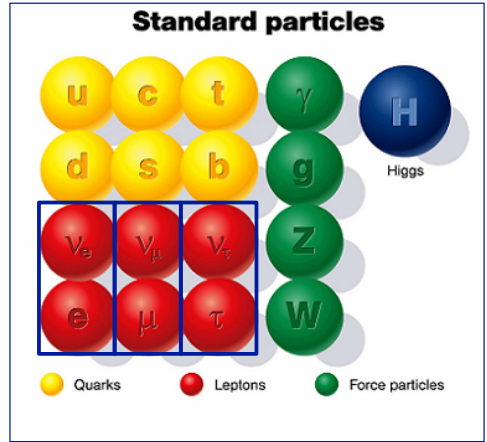
\includegraphics[scale=0.6]{Lezione13/zoo.png} 
\end{figure}
A parte la massa, la coppia $\mu-\nu_\mu$ ha le stesse proprietà di $e-\nu_e$. Per cui queste due coppie stanno nello stesso posto, mettono in evidenza la struttura a famiglie del \textbf{Modello Standard}. Quindi particelle che hanno la stessa proprietà cinetiche ma hanno la stessa differenza di massa. Il numero di particelle in una data famiglia è una quantità conservata. Nel 1975 venne scoperta la terza famiglia tau con il neutrino tauonico. $\tau-\nu_\tau$. La differenza di massa è ancora maggiore in quanto: $m_\tau=1776.82\pm0.16\,MeV$. La massa di tau avendo una massa maggiore del protone, quindi è un leptone che nei suoi decadimenti deboli non produce solamente muoni ed elettroni ma può produrre anche altri tipi di particelle cariche. 
\subsection{Osservazione del pione}
Il pione è stato difficile da osservare in quanto ha una vita media decisamente più piccola del muone. Per acquisire maggiori informazioni sui raggi cosmici furono fatti voli con palloni in alta atmosfera. Furono utilizzati emulsioni nucleari per registrare le interazioni. 
 %IMMAGINE pi
\begin{figure}[htp!]
  \centering
  
\includegraphics[scale=0.5]{Lezione13/pi.png} 
\end{figure}
Una pellicola fotografica contiene dei composti chimici che quando assorbono energia cambiano la struttura nucleare. Nel processo di lavorazione viene messo in evidenza, attraverso una colorazione diversa, le parti dove è stata ceduta energia. In questo caso vedo un pione che ad un certo punto decade. Dal decadimento si forma un muone fino a decadere in un elettrone. Come capiamo la freccia del tempo. Vediamo che la perdita di energia per ionizzazione è tanto più alta tanto più lenta la particella che si muove. Quindi quando vediamo una particella con una grande densità di energia, poi vediamo che una particella ha una densità di energia bassa fino ad aumentare sempre di più (traccia più marcata). E invece come faccio a risalire al tipo di particella? Il punto importante è che se vediamo una particella che parte veloce e poi si ferma si possono contare le interazioni avute. Integrando questo si calcola l'energia totale della particella. Poi sappiamo anche il $\beta^2$. In più le tracce non sono dritte ma presentano delle deviazioni. 

Questa nuova particella deve essere carica in quanto è osservabile nelle emulsioni nucleari. Esiste sia come particella positiva che negativa (basta includere un campo elettromagnetico nell'esperimento): $\pi^+$, $\pi^-$. La massa e la vita media: 
\begin{equation*}
    m_\pi=139.57108\pm0.00035\,MeV \qquad \tau_\pi=(2.6033\pm0.0005)\times10^{-8}s
\end{equation*}
e dalla vita media si intuisce che c'entra con il decadimento debole. Perchè per le interazioni forti ci aspettiamo ci aspettiamo altri valori. Guardando la quantità di moto e l'energia di decadimento si nota che il decadimento è in due corpi: il muone viene emesso con un momento fisso: $30\,MeV/c$ e quindi cinematicamente il decadimento deve essere in due corpi perchè quantità di moto determinato. Il fatto che il momento ha questo valore e la sua massa è di circa $140\,MeV$ si può calcolare che il rinculo è con una particella di massa nulla. E siccome non si vedono interazioni di $\gamma$, la particella neutra deve essere un neutrino:
\begin{equation*}
    \pi^-\to\mu^-+\Bar{\nu}, \quad \pi^+\to\mu^++\nu
\end{equation*}
\textbf{Il pione ha quindi spin intero}. Successivamente è stato anche osservato il $\pi^0$ neutro. Ha una massa minore ma una vita media estremamente minore:
\begin{equation*}
    m_{\pi0}=134.9766\pm0.0006\,MeV \qquad \tau_{\pi0}=(8.52\pm0.18)\times10^{-17}s \qquad \pi^0\to\gamma+\gamma
\end{equation*}
Con un decadimento elettromagnetico. Abbiamo tre particelle con masse molto simili. Vengono prodotte con uguale probabilità. Questo ci fa pensare che questa particella anch'essa rispetta la simmetria dovuta allo spin isotopico ma questa volta con $I=1$ in quanto è presente neutra, negativa e positiva. Quindi \textbf{tripletto di spin isotopico}. La differenza di massa tra i tre stati del pione è dovuta all'interazioni elettromagnetiche che sono diverse e che quindi rompono la degenerazione.
\subsection{Proprietà del pione}
I pioni possono venire prodotti in abbondanza in interazioni forti:
\begin{align*}
    p+p \rightarrow p+n+\pi^{+} \\  p+p \rightarrow p+p+\pi^0 \\ p+n \rightarrow p+n+\pi^0 \\  p+n \rightarrow p+p+\pi^{-} \\  p+n \rightarrow n+n+\pi^{+}
\end{align*}
Con energia di soglia di (es.:$p+p \rightarrow p+n+\pi^{+}$):
\begin{equation*}
    \sqrt{s}\ge m_p+m_n+m_\pi
\end{equation*}
Se voglio produrre una particella nello stato finale devo avere che nel sistema del centro di massa devo avere almeno energia sufficiente per avere la massa delle particelle coinvolte. Quindi nel sistema del centro di massa l'energia deve soddisfare questa condizione. Quindi
\begin{equation*}
    s\ge\left(m_p+m_n+m_\pi\right)^2=\left(m_p+m_n\right)^2+2\left(m_p+m_n\right) m_\pi+m_\pi^2 \approx 4 m_p^2+4 m_p m_\pi+m_\pi^2
\end{equation*}
\begin{equation*}
    s=\left(p_{p 1}+p_{p 2}\right)^2=m_p^2+m_p^2+2 m_p E_p=4 m_p^2+2 m_p T_p
\end{equation*}


$\begin{array}{lc}
& \qquad p_{p 1}=\left(\begin{array}{ll}E_p=m_p+T_p, & \mathbf{p}_p\end{array}\right) \\ T_p \geq 2 m_\pi\left(1+\frac{m_\pi}{4 m_p}\right) \approx 290 \mathrm{MeV} & p_{p 2}=\left(\begin{array}{ll}m_p, & \mathbf{0}\end{array}\right)\end{array}$

Vediamo che per produrre un pione che ha una massa di $140\,MeV$ ho bisogno di un protone quasi di due volte di quel valore. Questo perchè oltre all'energia bisogna conservare anche il momento. Oltre a questo se ho energia abbastanza grande posso produrre un numero più grande di pioni ad esempio:
\begin{equation*}
    p+p\to p+n+\pi^++\pi^0 \qquad p+p\to p+p+\pi^++\pi^-
\end{equation*}
Con energia di soglia di:
\begin{equation*}
    T_p \geq 4 m_\pi\left(1+\frac{m_\pi}{2 m_p}\right) \approx 600 \mathrm{MeV}
\end{equation*}
Quindi \textbf{il numero di pioni} diversamente dal numero di nulceoni \textbf{non viene conservato}. Quindi il numero barionico del $\pi=0$
\subsubsection{Spin}
Lo spin del pione è stato misurato sfruttando l'invarianza per \textbf{inversione temporale} delle \textbf{interazioni forti}, che permette di utilizzare il principio del \textbf{bilancio dettagliato} nelle reazioni. Posso verificare due condizioni: faccio un fascio di protoni, lo mando contro un bersaglio di idrogeno e misuro la sezione d'urto per la produzione di deuterio e del pione
\begin{equation*}
    p+p\to d+\pi^+
\end{equation*}
oppure produco un fascio di pioni lo lancio contro nuclei di deuterio e vedo la sezione d'urto dei protoni prodotti:
\begin{equation*}
    \pi^0+d\to p+p
\end{equation*}
La probabilità di transizione per unità di tempo sono date dalla regola d'oro di Fermi:
\begin{equation*}
    \lambda_{i\to f}=\frac{2\pi}{\hbar}|M_{i\to f}|^2\rho(E_f) \qquad \lambda_{f\to i}=\frac{2\pi}{\hbar}|M_{f\to i}|^2\rho(E_i)
\end{equation*}
L'invarianza per inversione temporale impone la condizione:
\begin{equation*}
    |M_{i\to f}|^2=|M_{f\to i}|^2
\end{equation*}
E ricordando il legame tra sezione d'urto $\sigma$ e $\lambda$:
\begin{equation*}
    \lambda_{i\to f}=\frac{\beta_ic}{d}\frac{1}{V}\sigma(i\to f)d
\end{equation*}
Dove $1/V$ è la sensità di bersagli: cioè una particella nel volume. Il flusso incidende come $v/d$. Numero di interazione per unità di tempo $dn/dt$ ma avendo una singola particella diventa proprio $\lambda$. E $d$ è la profondità del volume. 

Rispetto a quanto fatto in precedenza dobbiamo tenere conto dello spin negli stati finali: c'è una possibile degenerazione tra gli stati finali.
\begin{equation*}
    \rho\left(E_{\pi+d}\right)=\left(2 s_\pi+1\right)\left(2 s_d+1\right) \frac{V 4 \pi p_\pi^2}{(2 \pi \hbar)^3} \frac{d p_\pi}{d E_{\pi+d}}=\left(2 s_\pi+1\right) 3 \frac{V 4 \pi p_\pi^2}{(2 \pi \hbar)^3} \frac{d p_\pi}{d E_{\pi+d}}=\left(2 s_\pi+1\right) 3 \frac{V 4 \pi p_\pi^2}{(2 \pi \hbar)^3} \frac{1}{\beta_\pi c}
\end{equation*}
Tenendo conto che lo spin del deutone vale $s_d=1$. E soprattuto tenendo conto che $\mathrm{E}_{\pi+\mathrm{d}}=\mathrm{E}_\pi+\mathrm{E}_{\mathrm{d}}:$
\begin{equation*}
    \frac{d p_\pi}{d E_{\pi+d}}=\frac{d p_\pi}{d E_\pi} \qquad \frac{d p_\pi}{d E_\pi}=\frac{1}{\beta_\pi c}
\end{equation*}
Questa relazione vale sia nel caso relativistico che non relativistico.
Nel caso dello stato finale $p+p$, bisogna considerare che, avendo due \textbf{particelle identiche} non bisogna contare gli stati simmetrici, quindi lo stato deve avere una funzione d'onda asimmetrica.
\begin{equation*}
    \rho\left(E_{p+p}\right)=\frac{1}{2}\left(2 s_p+1\right)\left(2 s_p+1\right) \frac{V 4 \pi p_p^2}{(2 \pi \hbar)^3} \frac{d p_p}{d E_{p+p}}=\frac{1}{2} 2 \cdot 2 \frac{V 4 \pi p_p^2}{(2 \pi \hbar)^3} \frac{1}{\beta_p c}=2 \frac{V 4 \pi p_p^2}{(2 \pi \hbar)^3} \frac{1}{\beta_p c}
\end{equation*}
Ricordiamo la relazione per la sezione d'urto:
\begin{equation*}
    \sigma(i \rightarrow f)=\frac{V}{\beta_i c} \lambda_{i \rightarrow f}=\frac{V}{\beta_i c} \frac{2 \pi}{\hbar}\left|M_{i \rightarrow f}\right|^2 \rho\left(E_f\right)
\end{equation*}
Quindi se mettiamo insieme tutto quanto:
\begin{equation*}
    \sigma\left(p+p \rightarrow \pi^{+}+d\right)=\frac{2 \pi}{\hbar}\left|M_{p p \rightarrow \pi d}\right|^2 \frac{V}{\beta_p c} \rho\left(E_{\pi+d}\right)=\frac{2 \pi}{\hbar}\left|M_{p p \rightarrow \pi d}\right|^2 \frac{V}{\beta_p c}\left(2 s_\pi+1\right) 3 \frac{V 4 \pi p_\pi^2}{(2 \pi \hbar)^3} \frac{1}{\beta_\pi c}
\end{equation*}
\begin{equation*}
    \sigma\left(p+p \rightarrow \pi^{+}+d\right)=\frac{2 \pi}{\hbar}\left|M_{p p \rightarrow \pi d}\right|^2 \frac{4 \pi V^2}{\beta_p \beta_\pi c^2(2 \pi \hbar)^3}\left(2 s_\pi+1\right) 3 p_\pi^2
\end{equation*}
\begin{equation*}
    \sigma\left(\pi^{+}+d \rightarrow p+p\right)=\frac{2 \pi}{\hbar}\left|M_{\pi d \rightarrow p p}\right|^2 \frac{V}{\beta_\pi c} \rho\left(E_{p+p}\right)=\frac{2 \pi}{\hbar}\left|M_{\pi d \rightarrow p}\right|^2 \frac{V}{\beta_\pi c} 2 \frac{V 4 \pi p_p^2}{(2 \pi \hbar)^3} \frac{1}{\beta_p c} 
\end{equation*}
\begin{equation*}
    \sigma\left(\pi^{+}+d \rightarrow p+p\right)=\frac{2 \pi}{\hbar}\left|M_{\pi d \rightarrow p p}\right|^2 \frac{4 \pi V^2}{\beta_p \beta_\pi c^2(2 \pi \hbar)^3} 2 p_p^2
\end{equation*}
Facendo il rapporto tra le sezioni d'urto:
\begin{equation*}
    \frac{\sigma\left(p+p \rightarrow \pi^{+}+d\right)}{\sigma\left(\pi^{+}+d \rightarrow p+p\right)}=\frac{\left(2 s_\pi+1\right) 3}{2} \frac{p_\pi^2}{p_p^2}
\end{equation*}
Con questa relazione in mente si vanno a fare le misure della sezione d'urto:
 %IMMAGINE ss
\begin{figure}[htp!]
  \centering
  
\includegraphics[scale=0.5]{Lezione13/ss.png} 
\end{figure}
In questo grafico è la misura della sezione d'urto di $p+p\to\pi^++d$ in funzione dell'energia cinetica del protone e si vedono due tipi di pallini. Quelli neri sono dalla misura del nucleo diretto, quelli bianchi sono dati dalla misura della sezione d'urto del processo inverso moltiplicata per il fattore rapporto. Queste due sezione d'urto sono praticamente identiche. Quindi il termine $(2s_\pi+1)$ deve essere uguale a $1$. Dal confronto delle sezione d'urto quindi si ricava che $s_\pi=0$. Quindi usando il principio del bilancio dettagliato e di inversione temporale per misurare lo spin del pione. Questa è una delle tecniche possibili per fare misure di spin. 
\subsubsection{Parità}
La parità del $\pi$ si può determinare da reazione che lo contengono. Esempio:
\begin{equation*}
    \pi^-+d\to n+n
\end{equation*}
Questa reazione qui non ha una barriera coulombiana da superare (grazie alle cariche opposte). Quindi posso vedere  questa reazione per bassissimi momenti del pione: $p_\pi\to0$, quindi se il momento del pione è basso allora la reazione deve avvenire in uno stato di momento angolare $l=0$ avviene in onda $s$. Quindi il momento angolare orbitale è uguale a zero. A questo punto sappiamo che il momento angolare totale pione e deutone è $J=S_d$, $j=s_d=1$. La parità del sistema inziale è quindi:
\begin{equation*}
    \eta_\pi\eta_d(-1)^{l(\pi+d)}=\eta_\pi=1
\end{equation*}
Dato che $\eta_d=1$ e $l=0$.

Per quanto riguarda la parità del sistema finale. Qui entrano in gioco delle interazioni forti quindi la parità del sistema finale sarà uguale alla parità del sistema iniziale:
\begin{equation*}
    \eta_n\eta_n(-1)^{l(n+n)}=(-1)^{l(n+n)}
\end{equation*}
Lo stato contiene due particelle di spin $1/2$ identiche, la funzione d'onda deve essere anti-simmetrica. Sappiamo anche che il momento angolare totale $j=1$. Se $S(n+n)=0$, funzione d'onda di spin anti-simmetrica (appunto quando $s=0$). La funzione orbitale quindi deve essere simmetrica: quindi $l=0,2,\ldots$ pari. Ora con $l$ pari e $S=0$ non riesco a combinarli per avere $j=1$ perchè $j=l$. Quindi sappiamo che $S(n+n)=1$. Infatti la funzione d'onda di spin è simmetrica, quindi deve essere anti-simmetrica la funzione d'onda orbitale: $l=1,3,\ldots$. Quindi per avere $j=1$ se prendo $l=1$ ed $S=1$. Infatti il momento angolare totale in questo caso può essere 0, 1, 2. Quindi la parità dello stato finale è:
\begin{equation*}
    (-1)^l=-1
\end{equation*}
\textbf{La parità del pione è quindi negativa}.
\subsection{Decadimento del pione (carico)}
Nel sistema del centro di massa:
\begin{equation*}
    |\mathbf{p}_\mu^*|=|\mathbf{p}_\nu^*|=\frac{m_\pi^2-m_\mu^2}{2m_\pi} \qquad E^*_\nu=|\mathbf{p}_\nu^*|=\frac{m_\pi^2-m_\mu^2}{2m_\pi} \qquad E^*_\mu=\sqrt{m_\mu^2+\mathbf{p}_\nu^{*2}}=\frac{m_\pi^2+m_\mu^2}{2m_\pi}
\end{equation*}
Per valutare cosa succede nel sistema del laboratorio, prendiamo l'asse $z$ lungo la direzione di moto del $\pi$. L'angolo di decadimento nel sistema del centro di massa rispetto a tale direzione:
 %IMMAGINE ghj
\begin{figure}[htp!]
  \centering
  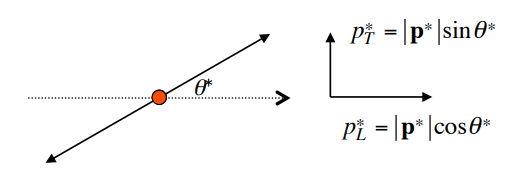
\includegraphics[scale=0.7]{Lezione13/ghj.png} 
\end{figure}
Se il pione si muove con velocità $\beta_\pi$:
\begin{align*}
     E_\nu=|\mathbf{p}_\nu|=\gamma_\pi\left(E_v^*+\beta_\pi E_v^* \cos \theta_v^*\right)=\gamma_\pi E_v^*\left(1+\beta_\pi \cos \theta_v^*\right)=\\
     =\gamma_\pi\left(1+\beta_\pi \cos \theta_v^*\right) \frac{m_\pi^2-m_\mu^2}{2 m_\pi}=\frac{\gamma_\pi m_\pi}{2}\left(1+\beta_\pi \cos \theta_v^*\right)\left(1-\frac{m_\mu^2}{m_\pi^2}\right)
\end{align*}
da cui segue che:
\begin{equation*}
    \frac{1-\beta_\pi}{2}\left(1-\frac{m_\mu^2}{m_\pi^2}\right)<\frac{E_v}{E_\pi}<\frac{1+\beta_\pi}{2}\left(1-\frac{m_\mu^2}{m_\pi^2}\right)
\end{equation*}
Per pioni relativistici:
\begin{equation*}
    0<\frac{E_v}{E_\pi}<1-\frac{m_\mu^2}{m_\pi^2}=0.428
\end{equation*}
Per calcolare la distribuzione di energie, basta osservare che in un decadimento istropo:
\begin{equation*}
    \frac{dN}{d\cos{\theta^*}}=\frac{1}{2}
\end{equation*}
Quindi la distribuzione di energia del neutrino è anch'essa uniforme:
\begin{equation*}
    \frac{dN}{dE_\nu}=\frac{dN}{d\cos{\theta^*}}\frac{d\cos{\theta^*}}{dE_\nu}\quad \cos{\theta^*}=\frac{E_\nu-|\mathbf{p}^*|\gamma_\pi}{|\mathbf{p}^*|\gamma_\pi\beta_\pi} \quad \frac{d\cos{\theta^*}}{dE_\nu}=\frac{1}{\gamma_\pi\beta_\pi|\mathbf{p}^*|}
\end{equation*}
Ricordando che:
\begin{equation*}
    |\mathbf{p}^*|=\frac{m_\pi^2-m_\mu^2}{2m_\pi}
\end{equation*}
Si ottiene che:
\begin{equation*}
    \frac{dN}{dE_\nu}=\frac{1}{|\mathbf{p}_\pi|\left(1-\frac{m_\nu^2}{m_\pi^2}\right)}
\end{equation*}
Se l'energia del pione è molto elevata è ragionevole approssimare:
\begin{equation*}
    E_\pi\approx|\mathbf{p}_\pi| \qquad \beta_\pi
\end{equation*}
Posto: $\xi=\frac{E_\nu}{E_\pi}$. [continua sulle slide].
\subsection{Il decadimento da pione a elettrone e neutrino}
Data l'esistenza del decadimento $\pi^+\to\mu^++\nu_\mu$ ci si aspetta anche l'analogo $\pi^+\to e^++\nu_e$ che effettivamente si osserva ma con un rapporto di decadimento molto minore:
 %IMMAGINE uy
\begin{figure}[htp!]
  \centering
  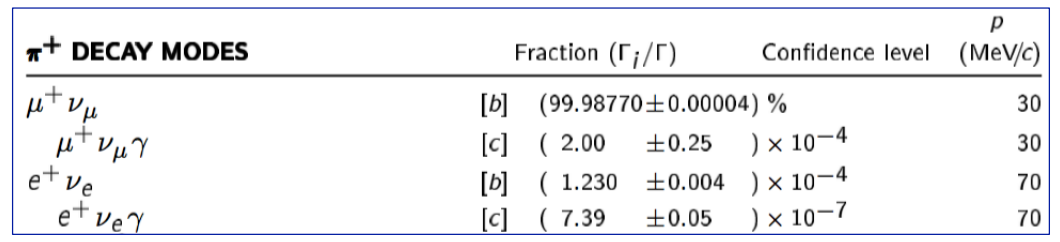
\includegraphics[scale=0.7]{Lezione13/uy.png} 
\end{figure}
Questa differenza è giustificabile dalla combinazione di: spazio delle fasi, conservazione del momento angolare e polarizzazione nelle interazioni deboli. Per quanto riguarda lo spazio delle fasi, che descrive il numero possibili di stati di energia di particelle nello spazio finale. Quindi si capisce che il decadimento tra pione e muone dove il Q valore (differenza di masse) è molto piccolo dell'ordine dei $40\,MeV$ avrà uno spazio delle fasi molto più piccolo rispetto a quello del decadimento in elettrone dove ci sono $140\,MeV$ a disposizione. Questo perchè lo spazio delle fasi dipende moltissimo dall'energia disponibile. Più energia ho disponibile più energia le mie particelle possono assumere combinazioni diverse. Lo spazio delle fasi quindi favorisce il decadimento in qualcosa di molto più leggero. Quindi questo termine favorisce il positrone.

Per quanto riguarda la consevazione del momento angolare: siccome il pione ha spin zero succede che per conservare il momento angolare gli spin delle due particelle emesse devono essere opposti. Le interazioni deboli sono in realtà delle cattive ragazze e cioè violano la parità. Uno degli effetti è che obbligano le particelle a favorire certe configurazioni di spin e quindi di elicità (quindi lo spin rispetto alla direzione di moto). In particolare il valor medio di ellicità di uno stato creato attraverso interazione debole ha come valor medio come elicità $-\beta=-\frac{v}{c}$. Mentre $\beta$ per le antiparticelle. Si dice quindi che le particelle sono left-hended e le antiparticelle sono right-hended Nei decadimenti $\beta$, $e^-$ e $\nu$ sono polarizzati con $\langle h \rangle=-\beta$ mentre le rispettive antiparticelle con $\langle h \rangle=+\beta$. Questo vuol dire che il leptone generico è in uno stato misto cioè è la somma di due funzioni una con spin allineato e uno antiallineato con i coefficienti che dipendono da $\beta$. 
\begin{equation*}
    \psi_l=a\psi_{h=+1}+b\psi_{h=-1}
\end{equation*}
con 
\begin{equation*}
    |a|^2=\frac{1+\beta}{2}\quad |b|^2=\frac{1-\beta}{2}
\end{equation*}
Nel decadimento $\beta$ l'interazione interagisce soltanto con la parte allineata come vuole l'interazione $\beta$ e quindi solo la componente antiparallela per le particelle e parallela per le antiparticelle.
Solo la componente con elicità negativa può contribuire.
 %IMMAGINE uy
\begin{figure}[htp!]
  \centering
  
\includegraphics[scale=0.3]{Lezione13/tt.png} 
\end{figure}

Quindi, ragionando un attimo qui vengono emesse un neutrino e un leptone. Il neutrino avendo massa piccolissima ha sempre $\beta=1$ quindi il neutrino esiste solo in uno stato. Esiste soltanto per forza con spin antiparallelo lungo la direzione di moto. Allo stesso modo l'antineutrino esiste soltato con spin parallelo alla direzione di moto. Da qui di fatto si porta alla teorizzazione che il neutrino possa essere l'antiparticella di se stessa. Proprio perchè il neutrino esiste solo antiparallelo e l'antineutrino esiste solo parallelo non è che sono la stessa particella in uno stato di elicità diverso? Questo ovviamente non posso dirlo per l'elettrone perchè per quanto questo preferisca essere lefthended c'è comunque una piccola percentuale che vuole esere righhended. Invece il neutrino che viene prodotto solamente nelle interazioni deboli e che interagisce quindi solamente con le interazioni deboli, la sua componente di polarizzazione opposta a quella che vorrebbe essere di fatto non esiste e non si osserva. Un problema che si sta ancora investigando. 

Ritornando a questo caso sul neutrino non abbiamo nessun margine di manovra. Il neutrino deve essere per forza antiparallelo. Lo spin della nostra particella originale è zero e quindi il nostro leptone si trova ad essere obbligato ad uno stato in cui non vuole e quindi lefthended(in questo caso perchè è un positrone). è obbligato anche lui ad avere uno spin parallelo ma ha effettivamente uno spin antiparallelo. Questo è concesso ma più il leptone è grande più il fattore $\beta$ è grande quindi è molto più facile che avvenga per il muone. Il decadimento in elettrone (positrone) è soppresso di un fattore $10^{5}$. Il termine dello spazio delle fasi lo favorirebbe ma a causa di questa cosa e cioè della violazione della parità (si dice violazione massimale della parità). Questa è una ulteriore prova dell'effettiva della violazione della parità nelle interazioni deboli.
\subsection{Risonanza e spin isotopico}
Dopo la scoperta del pione si osservano numerose risonanze nelle interazioni $N-\pi$ e $\pi-\pi$. Abbiamo visto che l'indipendenza della carica delle interazioni forti osservata nelle interazioni nucleone-nucleone. Ed il fatto che abbiamo particelle che compaiono in \textbf{multipletti} quasi degeneri: doppietto $p-n$, tripletto $\pi^+-\pi^--\pi^0$. Che sono stati che l'interazione forte non distingue. Porta alla formulazione dell'ipotesi di una \textbf{simmetria} delle interazioni per rotazioni in uno \textbf{spazio interno} delle particelle.  Queste risonanze possono venire analizzate a partire dalla simmetria di \textbf{isospin delle interazioni forti}. La simmetria non è esatta globalmente: viene ovviamente violata da interazioni elettromagnetiche e deboli. Differenze di massa spiegabili da effetti elettromagnetici. In base a questa simmetria è possibile classificare gli stati osservati aprendo la porta al modello a quark degli adroni.
\subsection{Ripasso: risonanze}
Ricordiamoci che possono esistere, quando facciamo collidere due funzioni d'onda, anche qua possono esistere delle risonanze. Viene fuori una formula fondamentalmente analoga alle risonanze classiche dove ciò che è risonante è la sezione d'urto.

Quando abbiamo visto la sezione d'urto in uno sviluppo di onde parziali: abbiamo preso la sezione d'urto, per poi la funzione d'onda scomponendola in onde incidente e onda che ha interagito con il potenziale in forma di onda sferica. Abbiamo visto che la sezione d'urto potevamo scriverla come sommatoria di diversi valori di momento angolare. Grazie a questo abbiamo potuto dire che la sezione d'urto è una sommatoria di termini con contributi di diversi momenti angolari con un $\delta_l$ che era lo sfasamento della funzione d'onda dopo l'interazione con il potenziale rispetto al caso di particella libera. Questo sfasamento mi da un'interferenza tra particella libera e interazione con il potenziale. Si dice che è la sezione d'urto scomposta in sezione d'urto parziali perchè mi ritrovo diversi contributi con i vari $l=0,1,\ldots$. Abbiamo già visto che ci può essere un valore massimo ed è un limite universale e non dipende dal potenziale. Questa $\delta_l$ varia con l'energia. Ricordo:
\begin{equation*}
    \sigma=\frac{\pi}{k^2}(2l+1)\sin^2{\delta_l} \quad (k=p/\hbar)
\end{equation*}
ed è massima per sfasamenti $\delta_l=\pm\pi/2$. Quando siamo in prossimità di questi massimi possiamo sviluppare nell'intorno con $\cot{\delta_l}$:
\begin{equation*}
    \cot{\delta_l}(E)=\cot{\delta_l}(E_R)+(E-E_R)\frac{\partial\cot{\delta_l}}{\partial E}+\ldots
\end{equation*}
Definendo:
\begin{equation*}
    \frac{\Gamma}{2}=\left(\frac{\partial\cot{\delta_l}}{\partial E}\right)^{-1}
\end{equation*}
Sostanzialmente se questa derivata è molto veloce (quindi passo da $\pi/2$ molto velocemente) questa quantità sarà piccola e ragionamento inverso. Se siamo in un caso in cui: $\Gamma<<E$ e quindi lo sfasamento cambia velocemente in prossimità di tale valore dello sfasamento:
\begin{equation*}
    \cot{\delta_l}(E)=\frac{E-E_R}{\Gamma/2}
\end{equation*}
Se adesso traduciamo questo in sezione d'urto:
\begin{equation*}
    \sin^2{\delta_l}=\frac{1}{1+\cot^2{\delta_l}}=\frac{1}{1+\frac{(E-E_R)^2}{\Gamma^2/4}}=\frac{\Gamma^2/4}{\Gamma^2/4+(E-E_R)^2}
\end{equation*}
che ricorda il profilo di una Lorenziana e quindi risente degli stessi effetti di risonanza che si vedono anche negli oscillatori e in altri processi. Si ottiene la \textbf{sezione d'urto risonante}:
\begin{equation*}
    \sigma=\frac{\pi}{k^2}(2l+1)\frac{\Gamma^2/4}{\Gamma^2/4+(E-E_R)^2}
\end{equation*}
Picco della sezione d'urto per un certo valore del momento angolare. Quello che succede è che ho una transizione molto veloce tra uno stato e l'altro. Ora se andiamo a vedere questo specifico problema ci si accorge che queste transizioni intorno agli sfasamenti massimi si hanno nel caso in cui la condizione di raccordo tra la funzione d'onda all'interno del potenziale e all'esterno mi porta delle sinusoidi molto grandi all'interno del potenziale. 
 %IMMAGINE dsa
\begin{figure}[htp!]
  \centering
  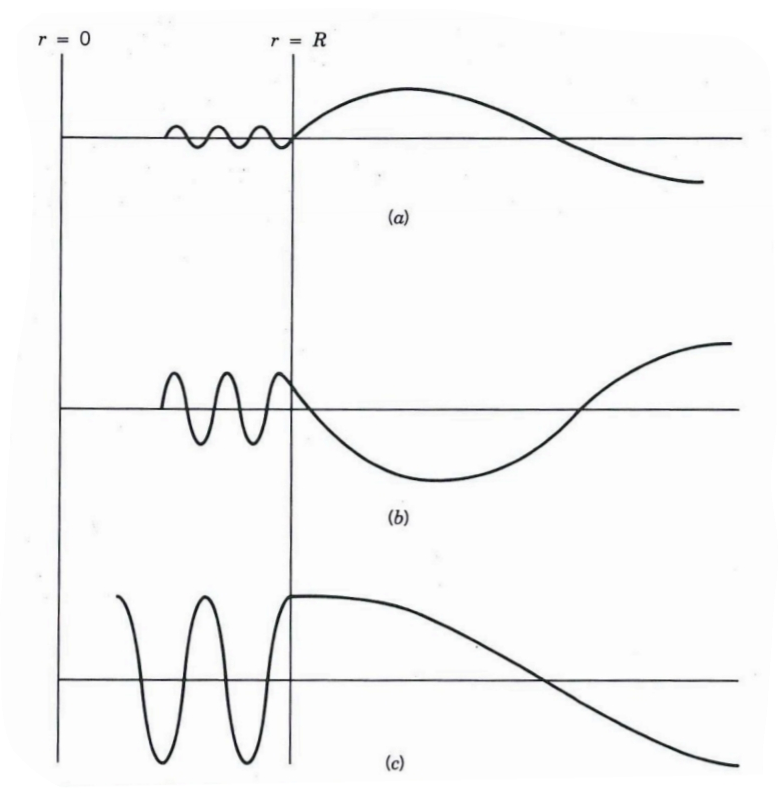
\includegraphics[scale=0.3]{Lezione13/dsa.png} 
\end{figure}
\subsection{Sezione d'urto e risonanze N-pione}
Ho scoperto il pione lo prendo e lo faccio collidere tra di loro e contro i nucleoni. Trovo che la probabilità di interazione non è piatta ma ha determinati picchi. Si nota che c'è un picco ad un ben specifico valore di $\sqrt{s}$ è cioè energia disponibile nel centro di massa. Questo picco stupisce. Questo mi dice che è molto più probabile avere interazione attorno a questo valore. Succede la stessa cosa quanto uso il pione negativo con il protone.
%IMMAGINE r1 r2
\begin{figure}[htp!]
  \centering
  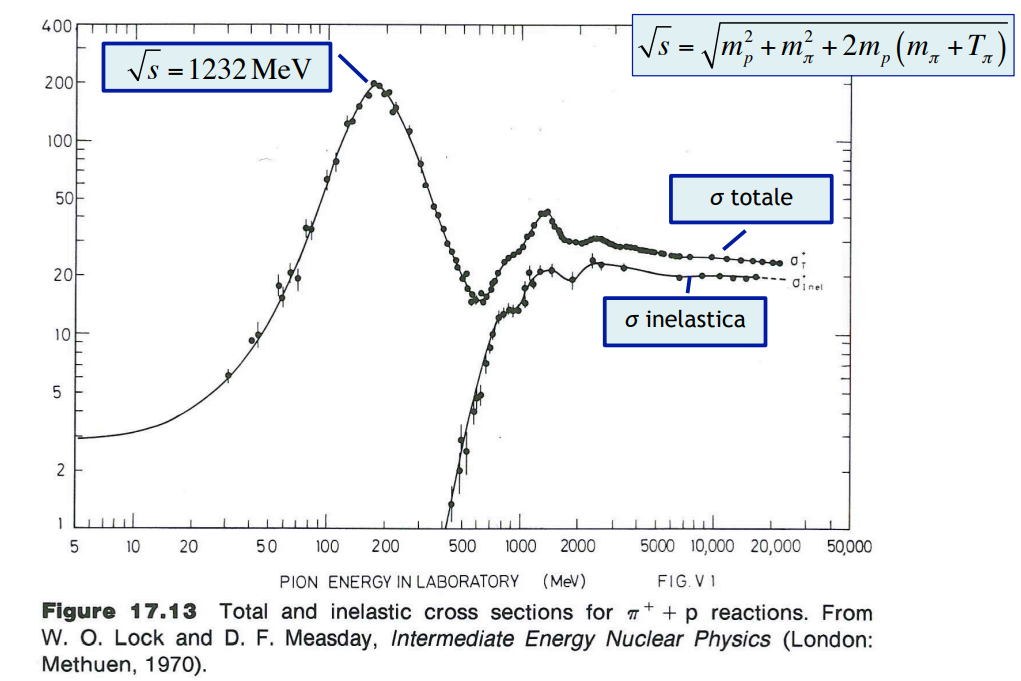
\includegraphics[scale=0.5]{Lezione13/r1.png}
  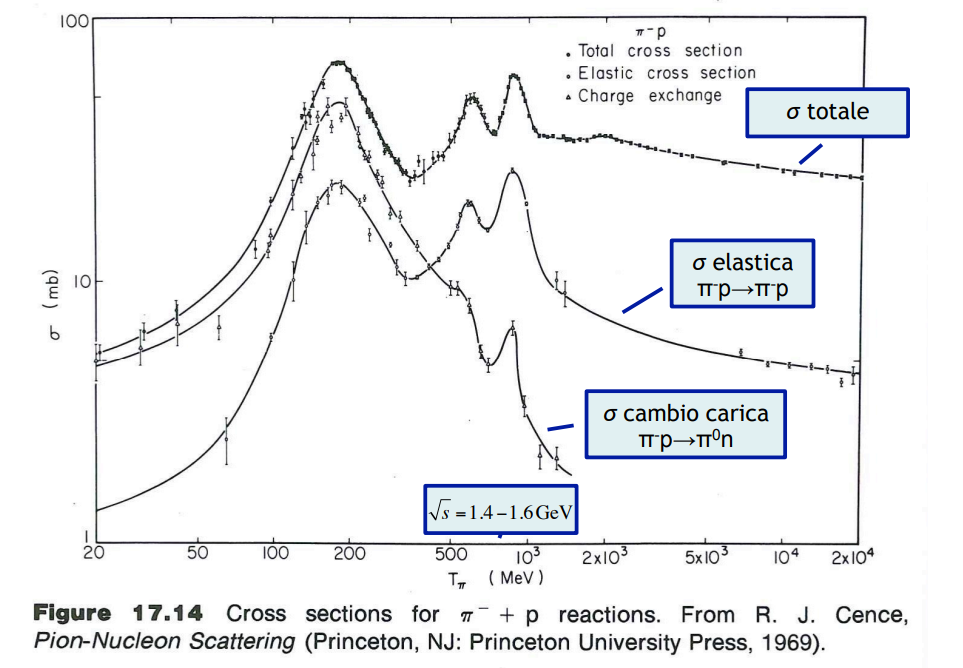
\includegraphics[scale=0.5]{Lezione13/r2.png} 
\end{figure}
In termini di spin isotopico $I$, uno stato ha molteplicità $2I+1$:
\begin{equation*}
    \mathrm{p}-\mathrm{n}: \mathrm{I}=1 / 2,|\mathrm{p}\rangle=\left|\mathrm{I}=1 / 2, \mathrm{I}_3=1 / 2\right\rangle \quad|\mathrm{n}\rangle=\left|\mathrm{I}=1 / 2, \mathrm{I}_3=-1 / 2\right\rangle 
\end{equation*}
\begin{equation*}
 \left.\Pi^{+}-\Pi^0-\Pi^{-}:|=1,| \Pi^{+}\right\rangle=\left|\mathrm{I}=1, \mathrm{I}_3=1\right\rangle\left|\Pi^0\right\rangle=\left|\mathrm{I}=1, \mathrm{I}_3=0\right\rangle\left|\Pi^{-}\right\rangle=\left|\mathrm{I}=1, \mathrm{I}_3=-1\right\rangle
\end{equation*}
Vale la formula di Gell-Mann-Nishijima:
\begin{equation*}
    Q=\frac{B}{2}+I_3
\end{equation*}
Dove $Q$ è la carica (in unità di $e$), $B$ il numero barionico ($1$ per i barioni, $-1$ per gli antibarioni e $0$ per i mesoni come il pione). Lo stato $\pi^+p$ è uno stato puro $I=3/2$: risonanze $\Delta$ (4 stati di carica). Lo stato $\pi^-p$ è uno stato misto. Quindi:
\begin{equation*}
    |\pi^-p\rangle=\sqrt{\frac{1}{3}}|I=3/2,I_3=-\frac{1}{2}\rangle-\sqrt{\frac{2}{3}}|I=1/2,I_3=-1/2\rangle
\end{equation*}
Possibili risonanze $\Delta(I=3/2)$ che $N(I=1/2)$
Le stesse cose valgono per i decadimenti infatti sono a tutti gli effetti delle particelle ma sono chiamate risonanze perchè hanno dei tempi di decadimento infinitesimi. Infatti anche se andassero alla velocità della luce percorrerebbero uno spazio infinitesimo. Come si calcola il tempo di decadimento di queste particelle? In che cosa decadono queste particelle? In base all'isospin decadranno in una cosa piuttosto che in un'altra.
\begin{equation*}
    |I=3/2,I_3=-\frac{1}{2}\rangle=\sqrt{\frac{2}{3}}|\pi^0n\rangle+\sqrt{\frac{1}{3}}|\pi^-p\rangle
\end{equation*}
\begin{equation*}
    |I=1/2,I_3=-1/2\rangle=\sqrt{\frac{1}{3}}|\pi^0n\rangle-\sqrt{\frac{2}{3}}|\pi^-p\rangle
\end{equation*}
I coefficienti ci dicono quanto pesa uno stato rispetto all'altro quindi facendo il primo esempio è molto più facile che il decadimento sia $|\pi^0n\rangle $ rispetto all'altro. Quindi nei grafici dovremmo osservare che il picco di risonanza è più alta quando vediamo quegli stati finali rispetto all'altro.
 %IMMAGINE hh
\begin{figure}[htp!]
  \centering
  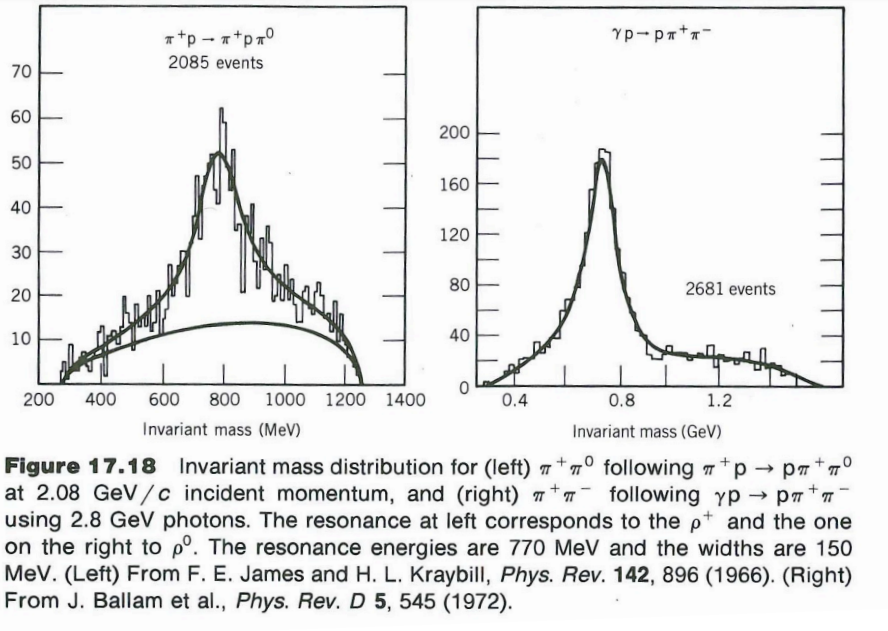
\includegraphics[scale=0.7]{Lezione13/hh.png} 
\end{figure}
Nell'esempio a sinistra quando vado a calcolare la mia massa invariante posso calcolarla soltanto per un sottopezzo. In questo caso di $\pi^+\pi^0$. In questa distribuzione trovo un altro picco di risonanza che però non può essere una $\Delta$ perchè questo è soltato $\pi^+\pi^0$ il numero barionico si deve conservare quindi ho una particella punto di domanda che mi viene prodotta in questa interazione che poi decade nei due mesoni. Quindi la particella punto di domanda non può essere una delta in quanto abbiamo visto che normalmente decade in protone e neutrone quindi deve avere numero barionico $=1$ quindi deve essere un barione. Mentre qui no. La particella punto di domanda la chiamiamo risonanza $\rho$ è un mesone ed ha quindi numero barionico uguale a zero. Altro modo per capire che non è una delta rimane solamente dal fatto che ha una massa diversa. Infatti ricordo che la $\Delta$ ha una massa di: $m_\Delta=1232\,MeV$. Mentre il mesone $\rho$ dalla figura di vede avere una massa di circa $m_\rho=776\,MeV$.

Allo stesso modo a destra vedo che dentro c'è un gamma. Quindi vedo come posso produrre queste risonanze non solo nelle interazioni forti ma anche in interazioni elettromagnetiche. Poi queste risonanze decadranno in maniera forte ma la produzione può anche derivare da interazioni diverse. Se ho un fotone ho per forza interazione elettromagnetica. Infatti ho un fotone a sinistra ma non un fotone a destra.
 
\subsection{Massa invariante}
La massa invariante di un sistema a due particelle $a+b$ è l'energia nel loro sistema del centro di massa. Si ottiene dal quadrato della somma dei rispettivi tetravettori:
\begin{equation*}
    m^2=(p_a+p_b)^2=m_a^2+m_b^2+2p_a\cdotp_b=m_a^2+m_b^2+2(E_aE_b-\mathbf{p}_a\cdot \mathbf{p}_b)
\end{equation*}
Nel caso si possa trascurare la massa a riposo delle particelle, si ha la reazione semplificata:
\begin{equation*}
    m^2=2E_aE_b(1-\cos{\theta_{a,b}})
\end{equation*}
Lo stesso principio di applica ad un sistema multi-particelle. Se le due particelle provendono da un detasimento di una particella madre: $C\to a+b$. Con questo metono si può mettere in evidenza la produzione di una nuova particella. $(p_a+p_b)^2=(p_c)^2=m_C^2$. Questo è anche il modo in cui si è visto il bosono di Higgs. Un picco nella distribuzione di massa invariante è centrato in $m_C$ con una \textbf{larghezza} dipendente dalla \textbf{risoluzione sperimentale} e dalla larghezza di decadimento $\Gamma_C$. Questo perchè $\Delta E\Delta t\ge\frac{\hbar}{2}$. Quindi noi non possiamo avere troppa precisione sul tempo, perchè ad esempio la particella mi decade troppo in fretta, questo degrata la precisione dell'energia. Ricordo che la massa invariante la posso fare per ogni sottogruppo di particelle che ho in gioco. Il punto è che mettiamo caso di avere un'interazione che mi produce 5 particelle. Io posso prenderle a coppie o a terne, fare la massa invariante e se io vado a vedere e trovo che c'è una risonanza in una di queste. Se pensavo in una interazione diretta in realtà è presente una particella che rinchiude le particelle di cui ho fatto la massa invariante che decade subito dopo:
\begin{equation*}
    X\to Y_1+ Y_2+ Y_3+ Y_4+ Y_5
\end{equation*}
Se faccio ad esempio la massa invariante tra $Y_4$ e $Y_5$ e noto una risonanza in realtà ho:
\begin{equation*}
    X\to Y_1+ Y_2+ Y_3+ (Z\to Y_4+ Y_5 )
\end{equation*}
Questo è anche il modo in cui è stato osservato il Bosone di Higgs.
\subsection{Altre risonanze}
Questo ad esempio è una risonanza addirittura quando vado a fare un'annichilazione tra elettrone e positrone dove al posto di produrre $\gamma$ vado a selezionare solamente quando vengono prodotti i due pioni
\begin{equation*}
    e^+e^-\to\pi^+\pi^-
\end{equation*}
Ancora una volta vedo un picco intorno a $780\,MeV$ guarda caso il picco esattamente nello stesso punto che era stato osservato in un altro processo. Quello in cui si faceva interagire un protone con pione. Quindi anche questa sarà una risonanza $\rho$. La larghezza è quella che mi dice il tempo di decadimento. La risonanza $\rho$ è un triplesso di isospin.
%IMMAGINE uy
\begin{figure}[htp!]
  \centering
  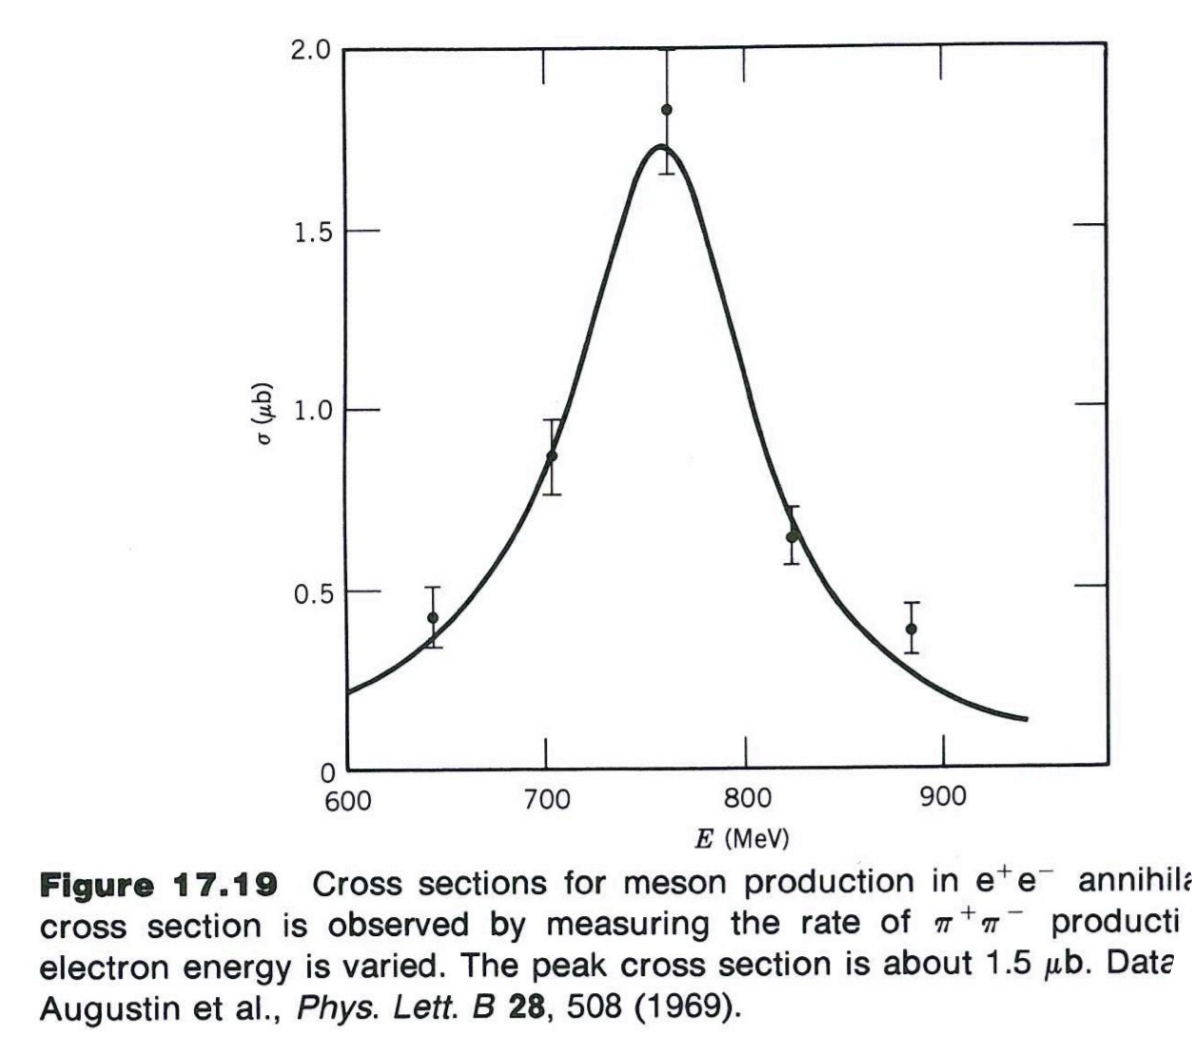
\includegraphics[scale=0.3]{Lezione13/hy.png} 
\end{figure}
%IMMAGINE uy
\begin{figure}[htp!]
  \centering
  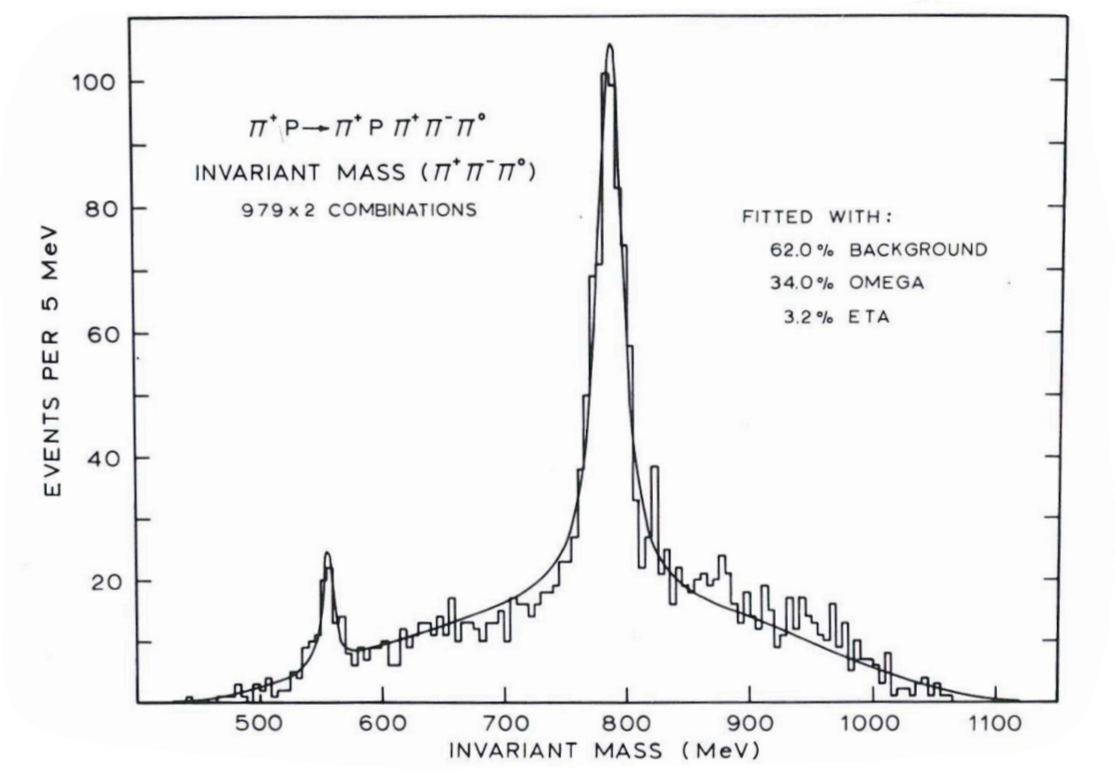
\includegraphics[scale=0.3]{Lezione13/uuu.png} 
\end{figure}
Esistono tantissime altre risonanze tra cui la $\eta$ e la $\omega$ che si notano quando si fa la massa invariante di tre pioni. Sotto si nota il fondo dovuto allo spazio delle fasi quindi di tutte le combinazioni possibili. Invece ci sono due risonanze e sono singoletti di spin isotopico. La risonanza $\eta$ può decadere solamente in $3$ pioni. Questo spiega perchè è strettina. Se è strettina significa che ha un tempo di decadimento relativamente lungo (per essere una particella che decade forte). Questo signigica che non ha molto spazio delle fasi perchè appunto può decadere solametne in tre pioni.  La risonanza $\rho$ al contrario può decadere in modi diversi quindi lo spazio delle fasi è più "popolato" quindi la risonanza è più larga e i tempi di decadimento più corti.
\subsection{Modello a Quark}
Il fatto che ci siano queste simmetrie fa capire che le particelle non sono poi così elementari. Ad esempio il positronio si comportano come stati legati. Si possono spiegare come stati legati di costituenti più elementari: \textbf{i Quark}. Esistono due quark in un doppietto isotopico: $S=\frac{1}{2}$, $B=\frac{1}{3}$ visto che mi ci vogliono tre quark per fare un barione. A questo punto la carica può essere $2/3$ quark up (u) con $I_3=1/2$ o $-1/3$ quark down (d) con $I_3=-1/2$ dalla formula:
\begin{equation*}
    Q=\frac{B}{2}+I_3
\end{equation*} 
Fa un po' strano vedere la carica come una frazione ma ce ne faremo una ragione in quanto i quark non possono vivere da soli. I barioni e i mesono sono quindi stati complessi: i barioni sono composti da 3 quark (infatti abbiamo $3\times1/3$ che rappresenta il numero barionico $B=1$), hanno spin semintero, hanno spin isotopico: $3/2$: risonanze $\Delta$ uuu (++), uud (+), udd (0), ddd (-). O $1/2$ nucleoni o risonanze $N$ uud (protone +), udd (neutrone carica 0).

I mesoni sono costituiti da una coppia quark-antiquark (infatti $1/3-1/3$ numero barionico $B=0$), hanno spin intero e nello stato fondamentale il momento angolare orbitale è nullo, spin del mesone è uguale alla somma degli spin dei due quark e spin isotopico: $I=1$ in cui ho $\pi$ e risonanza $\rho$. Oppure per $I=0$ per le risonanze $\eta$ e $\omega$ che abbiamo visto in precedenza. 